% vim: filetype=tex spell

%Helmholtz Cage

\chapter{Helmholtz Cage}

\label{ch:BG}

For the testing and calibration of the \ac{ACDS} it is useful to be to be able to create a controllable, uniform magnetic field.

\section{Hardware}

The Helmholtz cage was constructed in 2009 by the \ac{ARC} mechanical team. The cage consists of 3 pairs of concentric coils as shown in \cref{fig:helmholtz}. Each coil pair generates a nearly uniform magnetic perpendicular to the plane of the coil, together the three perpendicular coil pairs can generated a field in any direction.

\begin{figure}[!ht]
    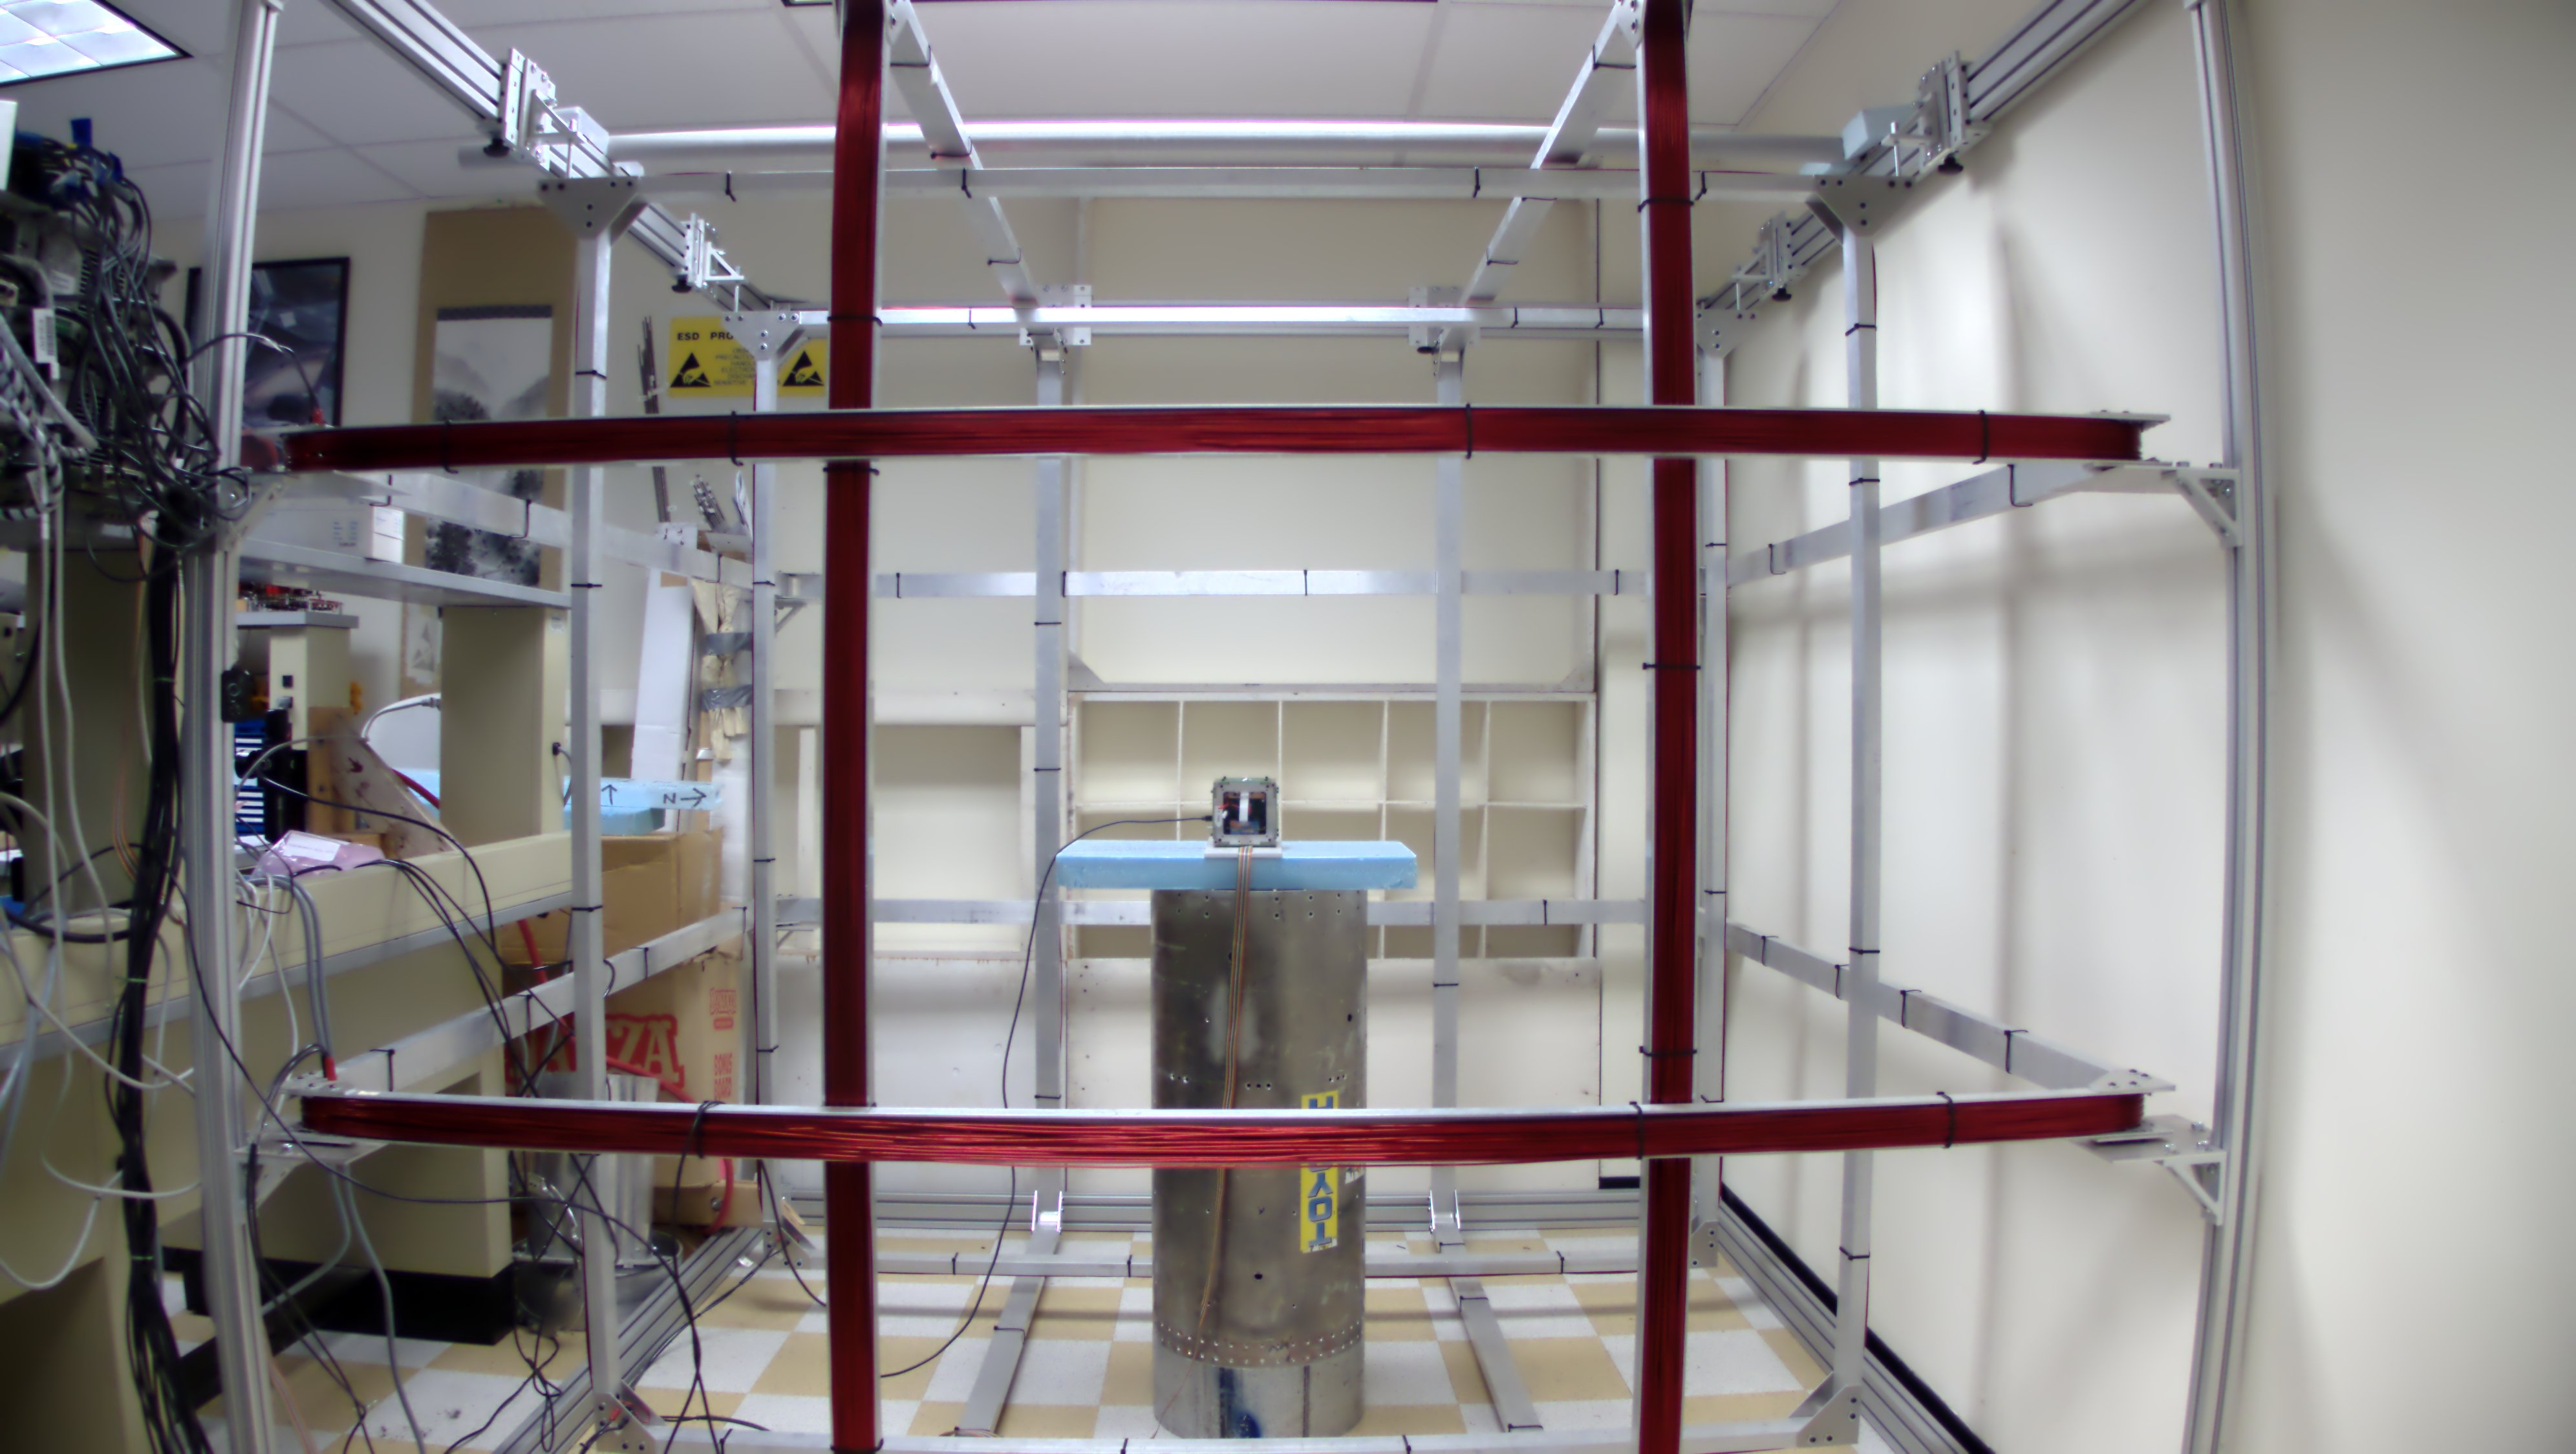
\includegraphics[width=\linewidth]{helmholtz-cage}
    \caption{The Helmholtz cage used for \acs{ACDS} testing}
    \label{fig:helmholtz}
\end{figure}

The coils are driven by a set of six Agilent E3633A power supplies as shown in \cref{fig:helmholtz-comp}. The power supplies have a maximum current of 20~A for output voltages less than 8~V or a maximum current of 10~A for output voltages of 20~V. The supplies are computer controlled with a \ac{GPIB} connection. 

An Alpha lab \#3AMG Milligauss Meter is used to measure the magnetic field of the Helmholtz cage. The meter is visible in \cref{fig:helmholtz-comp} to the left of the computer monitors. The Miligauss Meter has a digital display and an analog voltage output. The voltage output is read by a NI PCI-6010 Multifunction DAQ installed in the Helmholtz cage computer.

\begin{figure}[!ht]
    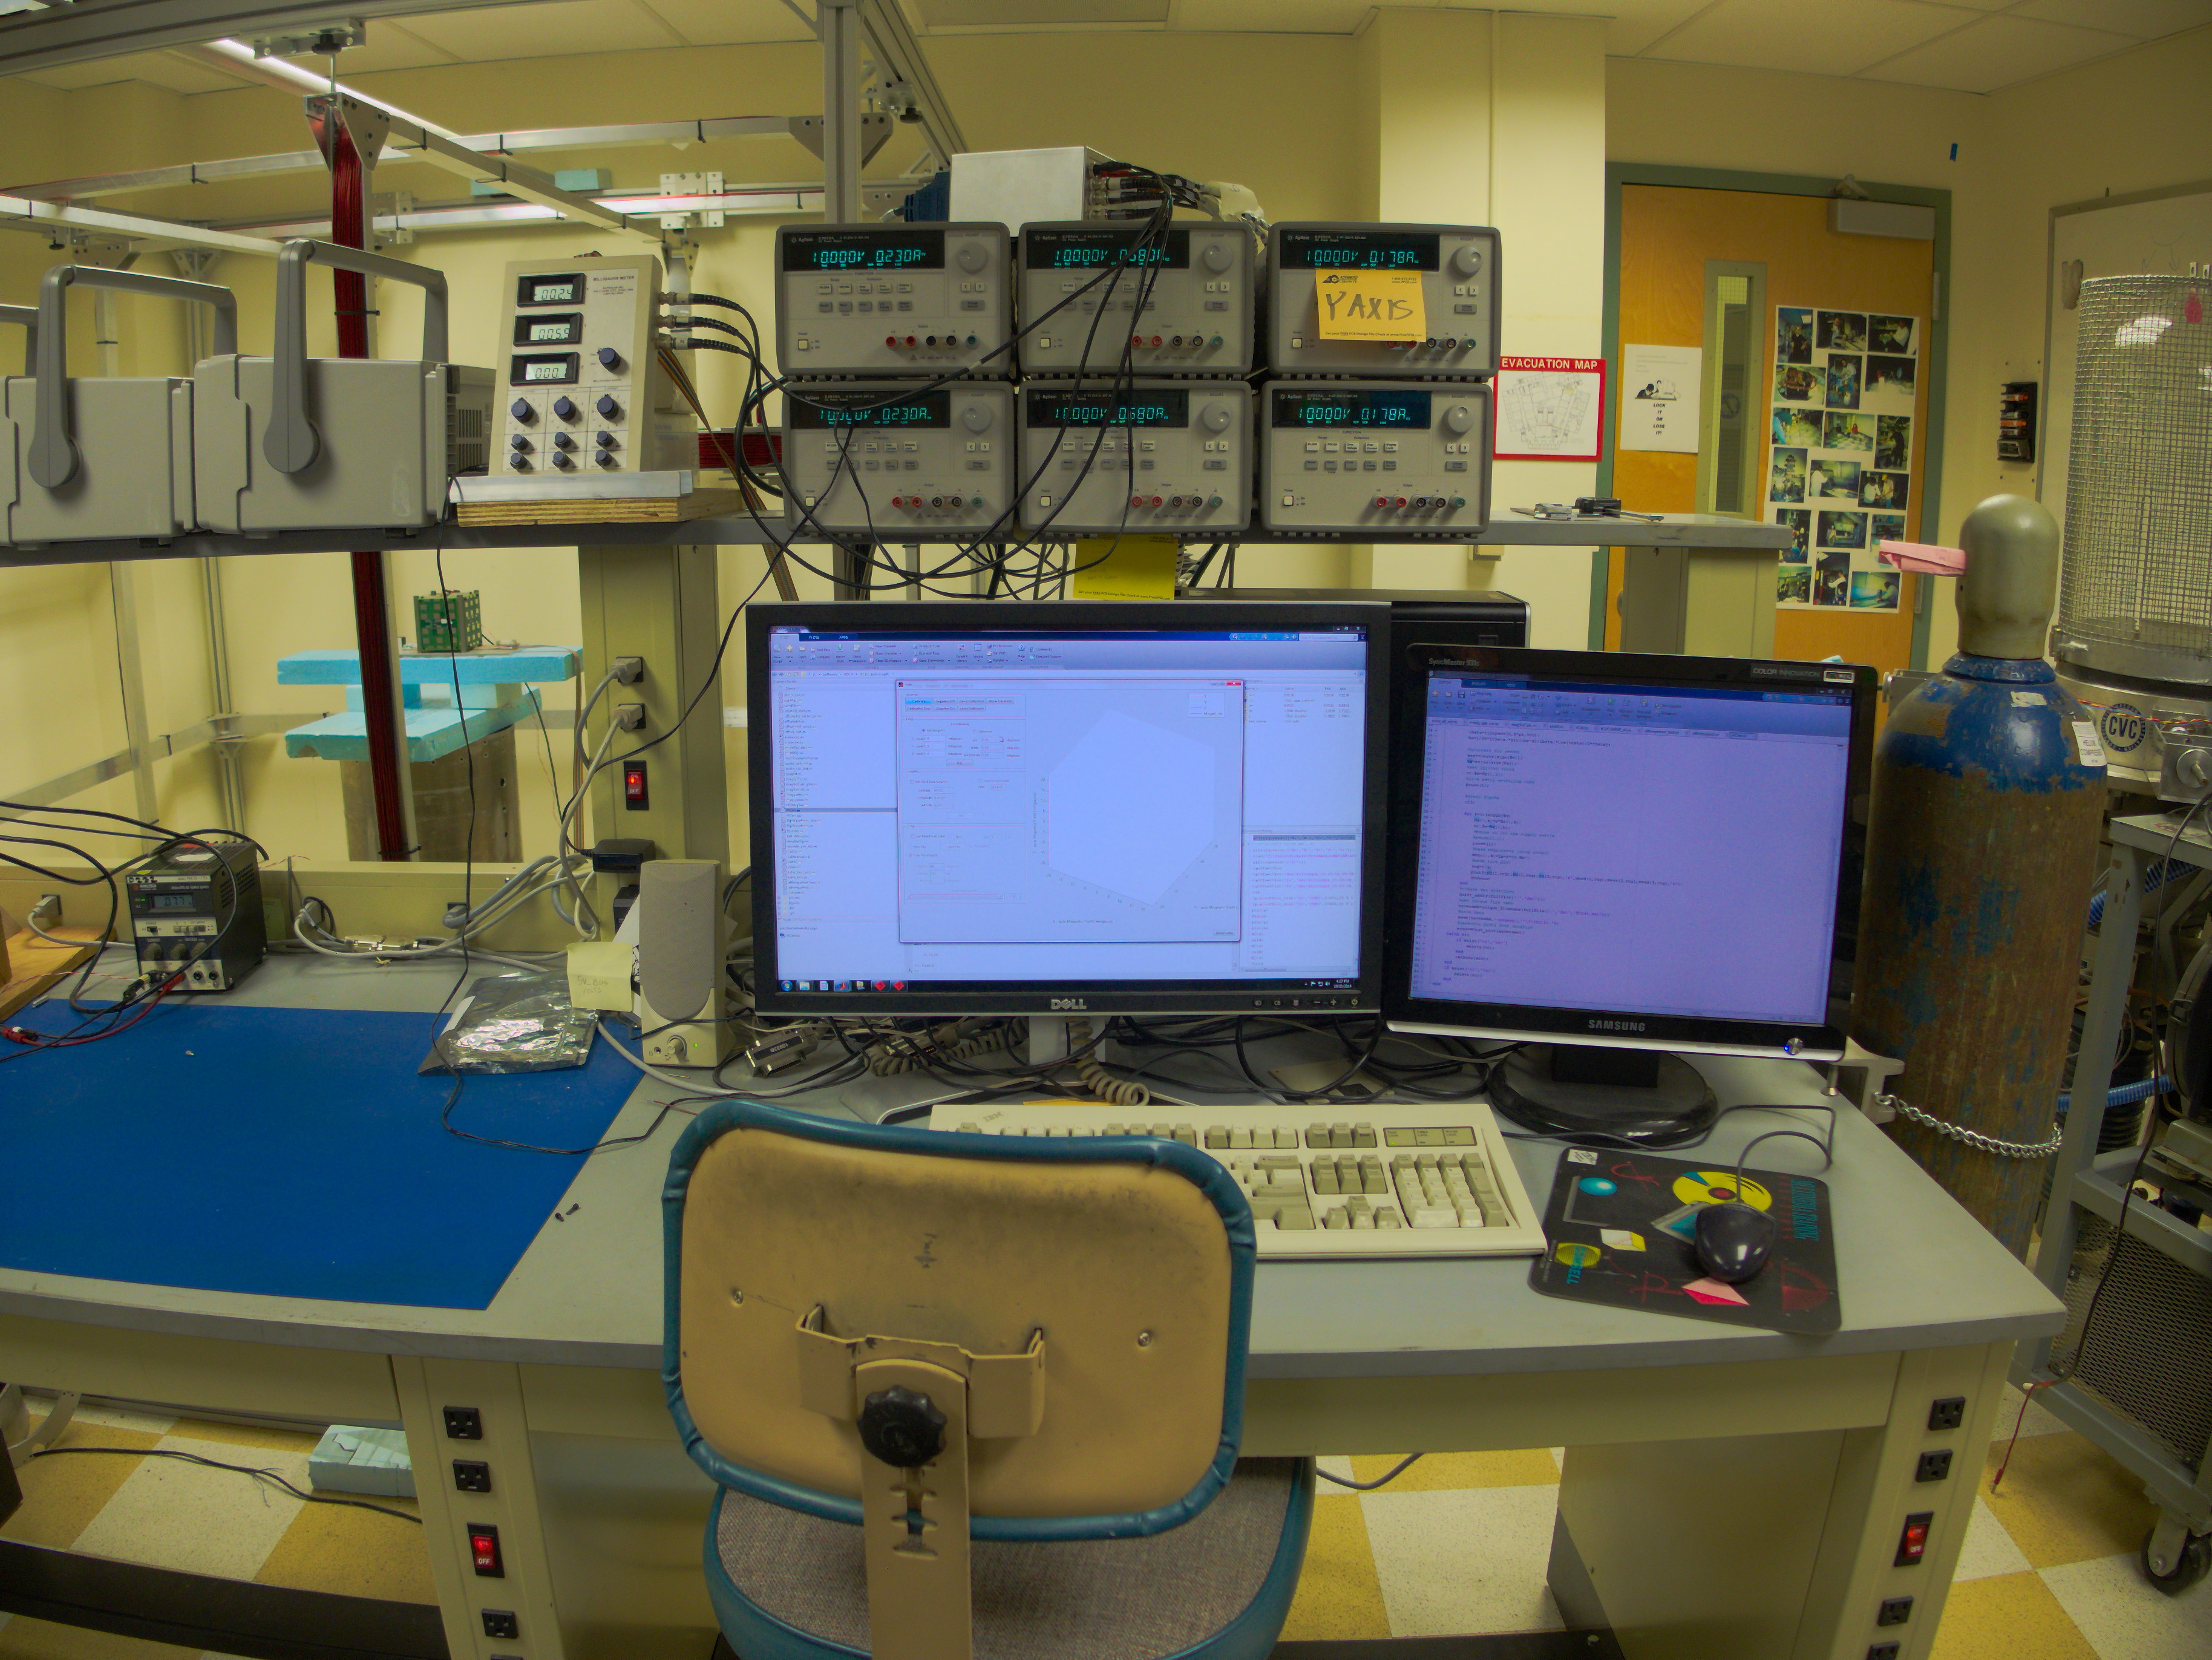
\includegraphics[width=\linewidth]{helmholtz-computer}
    \caption{The Helmholtz cage computer and power supplies}
    \label{fig:helmholtz-comp}
\end{figure}

\Cref{fig:hc-block} shows the block diagram of the Helmholtz cage. The cage control class is a \matlab class that is used for low level interfacing to the Helmholtz cage hardware. The \ac{GPIB} interface is used to connect to the power supplies. The power supplies are connected to the coils through the H-bridge so that the current direction can be reversed. The H-bridge is controlled using the digital I\textbackslash{}O on the DAQ card. The magnetometer is connected to the analog input channels of the DAQ and reads the magnetic field in the Helmholtz cage. 

\begin{figure}[!ht]
    % We need layers to draw the block diagram
    \pgfdeclarelayer{background}
    \pgfdeclarelayer{foreground}
    \pgfdeclarelayer{Hardware}
    \pgfdeclarelayer{CPU}

    \pgfsetlayers{background,Hardware,CPU,main,foreground}

    \begin{tikzpicture}[node distance = 6mm, auto]
        \node[prog,text width=2.2cm]     (cc)    {cage\_control class};
        \node[perif,right=of cc]      (gpib)  {\rotatebox{90}{\acs*{GPIB}}};
        \node[perif,above=of cc]      (daq)   {DAQ};
        \node[hardware,right=of gpib] (ps)    {Power Supplies};
        \node[hardware,right=of ps]   (dir)   {H-bridge};
        \node[hardware,right=of dir]  (coils) {Helmholtz Coils};
        \node[hardware,above=of daq]  (mag)   {Three-axis Magnetometer};

        \node[prog,text width=2.2cm,left=of cc]       (user)   {User Application};

        \begin{pgfonlayer}{CPU}
            \node (push) at ([yshift=-1cm,xshift=-4mm]user.south west) {};
            \node[CPU,fit=(cc) (gpib) (daq) (push) (user)] (cpu) {};
            \node[above,anchor=south west] at (cpu.south west) {Helmholtz cage computer};
        \end{pgfonlayer}

        \path[dataL] (cc) -- (daq);
        \path[dataL] (daq) -- (mag);

        \path[dataL] (cc) -- (gpib);
        \path[dataL] (gpib) -- (ps);

        \path[dataL] (user) -- (cc);

        \path[powerL] (ps) -- (dir);
        \path[powerL] (dir) -- (coils);

        \path[phconn] (coils) |- (mag);
        \path[dataL] ([xshift=2mm]daq.north) -- ++(0,2mm) -| (dir);

    \end{tikzpicture}
    \caption{Helmholtz cage software block diagram}
    \label{fig:hc-block}
\end{figure}

The feedback from the magnetometer is used to calibrate the Helmholtz cage. The cage is calibrated by setting the power supplies to a range of currents and reading back the magnetic field. The data is then used to compute a $4\times4$ transformation matrix to get from current to magnetic field. The magnetometer is not used in a closed loop fashion because magnetic fields produced by a device under test would change the magnetic field giving erroneous results.

The cage control class takes care of all of the low level hardware interaction and calibration for the Helmholtz cage. The cage control class opens interface objects to the power supplies and the DAQ. 

